\chapter{RESULTS}

We modified the published codes of the layer decomposition and MSERs, which are available on GitHub (at:https://github.com/CraGL/Decompose-Single-Image-Into-Layers; and https://github.com/idiap/mser),the differences between our algorithm and the available codes have been explain in Section 4.2.1 and 5.2. We performed the proposed approach on eight brush paintings, including Rosemaling and Chinese brush paintings. All the paintings are from the internet. Compared to Rosemaling, Chinese brush paintings do not emphasize the use of vibrant colors, even the adjacent strokes may share the same color in some paintings. The boundary of the overlapped brush strokes may be very blurred. Thus, we select some of the Chinese brush paintings for a test in terms of the boundary of strokes and the use of transparency. All the tests were performed on a 6-core of 3.33 GHz Intel Core Xeon CPU with memory of 32 GB(RAM).
In our implementation, the parameters in Layer decomposition, ETF field, and MSERs are set the default values as in the original codes. Table 2 further shows the running time of the proposed approach. Compared to the performance in \cite{tan2016decomposing} and \cite{nister2008linear}, there is no distinct difference. Additionally, SFS does not consume much time since it depends on the segmented stroke regions. Our implementation is not multithreaded. All the resulting images are available in the next section.  

\begin{figure}[H]
	\centering
	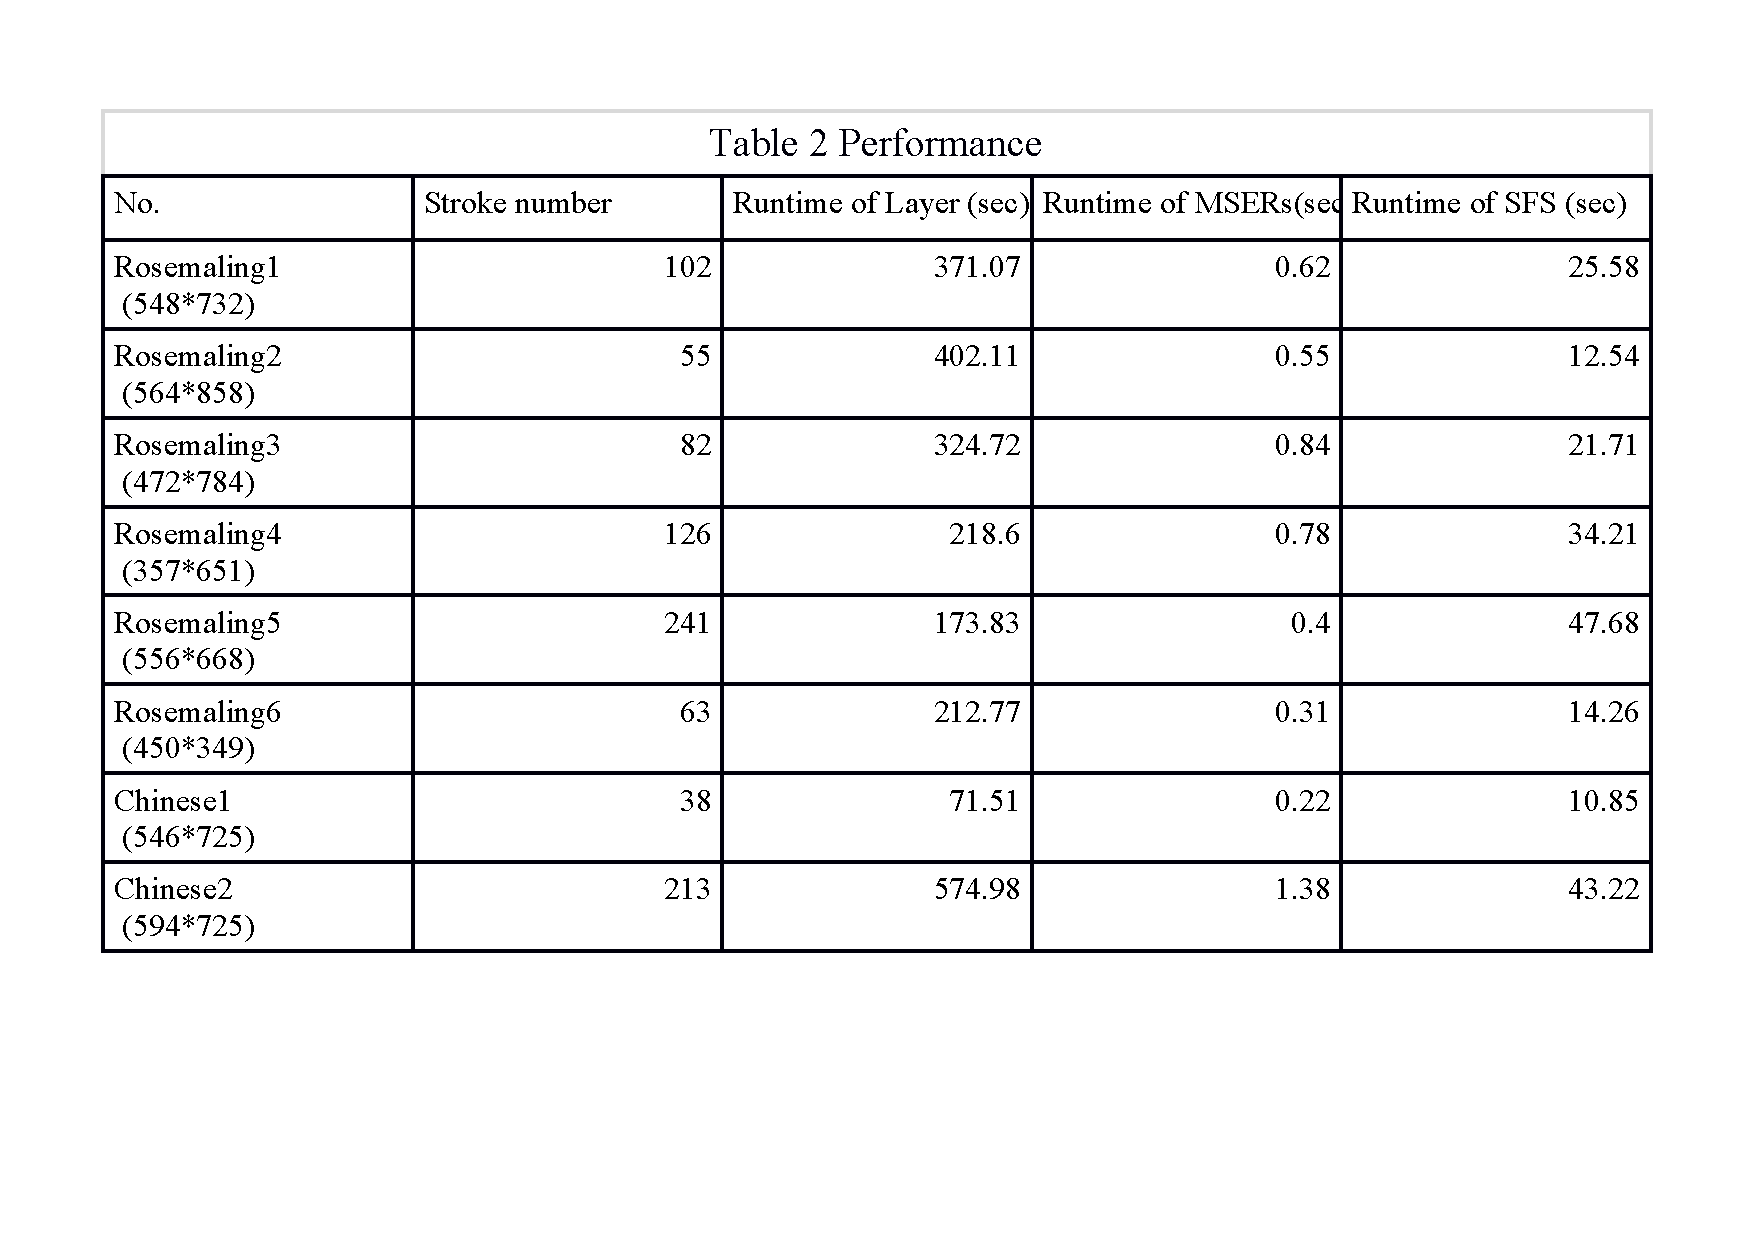
\includegraphics[width=15cm]{performance.pdf}

\end{figure}


